\documentclass[11pt,a4paper]{article}

\usepackage[margin=1in]{geometry}
\usepackage{times}
\usepackage{amsmath,amssymb}
\usepackage{booktabs}
\usepackage{graphicx}
\usepackage{xcolor}
\usepackage{hyperref}
\usepackage{enumitem}
\usepackage{caption}
\usepackage{subcaption}
\usepackage{tabularx}
\usepackage{array}
\usepackage{microtype}
\usepackage[numbers,sort&compress]{natbib}
\usepackage{fancyhdr}
\usepackage{titlesec}

\hypersetup{
  colorlinks=true,
  linkcolor=black,
  citecolor=blue!50!black,
  urlcolor=blue!50!black,
  pdftitle={Transfer-Stable Collusion Representations},
  pdfauthor={Andy Liang}
}

\pagestyle{fancy}
\fancyhf{}
\fancyhead[L]{\small Transfer-stable collusion representations}
\fancyhead[R]{\small Andy Liang · weekend review}
\fancyfoot[C]{\thepage}
\renewcommand{\headrulewidth}{0.4pt}

\title{\textbf{Transfer-Stable Collusion Representations in Multi-Agent\\
Committee Models:\\[0.3em]
\large J-Space Failure, Attention Localization, and Causal Humility}}
\author{Andy Liang\\[0.4em]
{\normalsize\textit{NARCBench Transfer-stable lane · Gemma-2-9B-it · weekend research review}}\\[0.2em]
{\normalsize\texttt{andy-biz/papers/transfer-stable-collusion-2026-10}}}
\date{1 October 2026 (PT)}

\begin{document}
\maketitle

\begin{abstract}
Prior NARCBench-style work shows that full residual / activation probes can separate colluding from non-colluding agents in multi-agent committee games---often near ceiling in-distribution. That establishes \emph{monitorability} of collusion from hidden state, but leaves open where the signal lives (verbalizable / J-space versus complement), whether a shared direction transfers across scenario families (Core$\to$Transfer), whether the geometry is role/deception-specific or entangled with run-level setup, and whether the direction is editable.

This weekend review consolidates a \textbf{mechanism follow-on} on Gemma-2-9B-it. Correlational results (facts only): HARD Transfer primary AUROC for full residual band L19--23 is \textbf{0.902}; W\_U / Jacobian $k{=}25$ J-only arms are weak (\textbf{0.602} / \textbf{0.549}) while complements match full (\textbf{0.898} / \textbf{0.891}); residual peaks at L21/L22 (\textbf{0.941} / \textbf{0.930}); attention residual-write at L22 reaches \textbf{$\approx$0.999}; low-rank contrast PCA ($k{\approx}4$--$8$) matches or beats ambient. Role and mode directions cross-predict (mode$\to$role $\approx$0.90; $\cos\approx$0.70); after residualizing mode, role still transfers (L21 0.859$\to$0.796). Causal free-regen last-token ablations on $n{=}6$ smokes were \textbf{null} across residual $\alpha$ sweeps and attn\_L22 final/discussion arms---so readability $\neq$ control under tested divergent-history edits. Science-freeze robustness (facts from \texttt{WEEKEND\_REVIEW}): Core discussion $\to$ Transfer \textbf{discussion} residual band primary \textbf{0.959}, attn\_L22 discussion \textbf{0.997}; Core domain-holdout @ L21 mean primary \textbf{0.939} (vs full-fit 0.941); all six Transfer families show strong Peak/Split @ L21.

\textbf{Claim we endorse:} a monitorable, Transfer-stable, mostly non-J coordination signature (attn\_L22 / mid-band residual). \textbf{Claim we refuse:} that scrubbing it is an off-switch, or that free-regen nulls prove epiphenomenality. Next science is matched-prefix interchange and within-trajectory assays, not residual-$\alpha$ chasing.
\end{abstract}

\tableofcontents
\vspace{0.5em}
\noindent\rule{\textwidth}{0.4pt}

\section{Introduction / problem}
\label{sec:intro}

Multi-agent language-model systems can collude: agents privately coordinate toward a shared target while presenting honest-looking public discussion. Safety work needs both \emph{detection} (is this committee in a collusive configuration?) and, ideally, \emph{intervention} (can we edit the responsible representation?). Rose et al.~\cite{rose2026narcbench} and related NARCBench-family protocols show that linear probes on full residual activations separate colluding versus non-colluding structure---often near ceiling when train and test share the Core distribution. That is an existence result for linear readout. It is not yet a mechanism result.

Probe-only papers leave four gaps that matter for monitoring and for claims about ``collusion circuits'':

\begin{enumerate}[leftmargin=1.4em,itemsep=0.25em]
\item \textbf{Where} in representation space? A verbalizable / logit-lens (J-space) story is attractive for interpretability narratives~\cite{nostalgebraist2020logitlens,belrose2023tunedlens}, but Transfer OOD may live elsewhere.
\item \textbf{What transfers?} In-distribution AUROC does not imply a Core-fit direction monitors held-out Transfer families.
\item \textbf{What is the geometry of?} Colluder-versus-honest \emph{role} may entangle with collusion-run versus control-run \emph{mode}---a coordination / setup state rather than a pure lying atom.
\item \textbf{Editable?} Classical causal tracing and activation patching~\cite{meng2022rome,geiger2021causal,turner2023activation} require matched computation; free regeneration with divergent histories is a weak test.
\end{enumerate}

This document is a \textbf{weekend-length research review} of the Transfer-stable lane on Gemma-2-9B-it~\cite{gemma2}: Core discussion-public train $\to$ Transfer final eval. It is not a re-run of the full-activation baseline. Soft-stops for this write-up: no Track~I / Paper~2 / interp-demo work; no new GPU; all numbers copied from existing artifacts under \texttt{results/transfer\_stable/} (including locked \texttt{WEEKEND\_REVIEW/CLAIMS\_NUMBER\_SHEET}) and HARD Transfer metrics. Causal GPU on the free-regen harness is paused pending matched-prefix redesign. Track~I remains soft-stopped.

\paragraph{One-line motivation.}
\emph{Can we locate a Transfer-stable coordination signature beyond ``full acts AUROC is high,'' and is it the sort of thing a safety monitor could claim---or only a probe?}

\section{Setup}
\label{sec:setup}

\subsection{NARCBench Core and Transfer}

\textbf{Core} is the in-distribution committee protocol family (multiple domains; letter \texttt{target\_option} available). \textbf{Transfer} is a held-out family set (six families in the FULL cache: \texttt{cicd}, \texttt{code\_review}, \texttt{news}, \texttt{pump\_dump}, \texttt{rag}, \texttt{research}). Agents play Peak / Split / Asymmetry scenarios under collusion or control conditions.

\paragraph{Model.}
\texttt{google/gemma-2-9b-it}~\cite{gemma2}. Hidden size $d{=}3584$. Cached residual layers for this lane: L19--L23 (last-token generation-time activations).

\paragraph{Activation caches (inventory summary).}
\begin{itemize}[leftmargin=1.2em,itemsep=0.15em]
\item Core residual: 1700 rows $\times$ 3584 at L19--23 (100 runs / 400 agents; discussion / private / final phases).
\item Transfer residual FULL: 936 rows $\times$ 3584 at L19--23 (72 runs / 288 agents).
\item MLP / attention residual-write extracts at matched layers (later in the lane).
\item J-basis: W\_U unembed ($k{=}25$ projections) and rank-64 sketched Jacobians at L19/21/23.
\end{itemize}
Canonical paths and caveats: only gen-time \emph{last-token} residuals (no tokenwise trajectory caches); Transfer \texttt{collusion\_success} is all-false in metadata---analyses use \textbf{mode} and \textbf{role} labels, never Transfer success as a class label~\cite{rose2026narcbench}.

\subsection{Phases, labels, metrics}

\begin{description}[style=nextline,leftmargin=1.2em,font=\normalfont\bfseries]
\item[Train protocol] Core \textbf{discussion public} turns; fit colluder-versus-honest within collusion runs (role), or run-level mode as needed.
\item[Eval protocol] Transfer \textbf{final} phase; zero-shot shared Core-fit direction / probe. HARD $n{=}72$ unless noted.
\item[mode] Collusion-run versus control-run (episode setup).
\item[role] Colluder versus honest agent (within-episode deception / coalition membership).
\item[Primary AUROC] Mean of Peak, Split, and Asymmetry scenario AUROCs (HARD Transfer tables).
\item[J-space] Span of top-$k$ logit-lens / unembed (W\_U) or Jacobian-aligned directions; \textbf{complement} is the orthogonal residual.
\item[attn / mlp / residual] Attention block residual-write (self-attn out), MLP residual-write, and DecoderLayer residual out, respectively. ``attn\_L22'' means the attention \emph{block output}, not a named head.
\end{description}

\section{Hypotheses, predictions, and falsifiers}
\label{sec:hypotheses}

Pre-registered flavor; tested against existing numbers (Table~\ref{tab:hypotheses}).

\begin{table}[t]
\centering
\caption{Hypotheses and status from this lane.}
\label{tab:hypotheses}
\small
\begin{tabular}{@{}cp{3.6cm}p{3.8cm}p{3.6cm}@{}}
\toprule
\textbf{\#} & \textbf{Hypothesis} & \textbf{Prediction if true} & \textbf{Status} \\
\midrule
H1 & Collusion signal is J-localized & J-only Transfer AUROC $\approx$ full; complement weak & \textbf{Rejected on Transfer} --- J-only weak; complement $\approx$ full \\
H2 & Shared residual direction transfers Core$\to$Transfer & Core-fit LR / low-rank subspace beats J-only; approaches full & \textbf{Supported} --- LR band $=$ full; contrast-PCA $k{\approx}4$--$8$ best \\
H3 & Signal peaks mid-band; attn write may dominate MLP & L21--L22 residual strong; attn $>$ mlp at matched layers & \textbf{Supported correlationally} --- L21/L22 best residual; attn\_L22 $\approx$0.999 \\
H4 & Direction is role-specific, orthogonal to mode & Role$\to$role high; mode$\to$role $\approx$ chance; $\cos\approx 0$ & \textbf{Rejected / mixed} --- both hit both; $\cos\approx 0.70$; residualize partially helps \\
H5 & Ablating role at last-token residual/attn steers votes & Ablate drops success / flips vs baseline \& random & \textbf{Not supported} under tested free-regen smokes ($n{=}6$ nulls) \\
\bottomrule
\end{tabular}
\end{table}

Core in-distribution was already easy (prior Stage-1 HARD\_PASS primary 1.0; J and complement both near-full on Core). The scientifically interesting cut is \textbf{Transfer OOD} + \textbf{specificity} + \textbf{causal editability}.

\section{Methods}
\label{sec:methods}

\subsection{Probes and shared directions}

Default eval script path: train logistic / direction on Core discussion public, score Transfer final. Arms include:

\begin{itemize}[leftmargin=1.2em,itemsep=0.15em]
\item Full residual acts (per layer L19--23; band mean; mean-pool).
\item Diff-in-means (colluder $-$ honest) unit vector.
\item Logistic-regression (LR) weight vector (same fit protocol as the ambient probe).
\item PCA on residual activations ($k\in\{1,2,4,8,16,32\}$) and PCA on colluder$-$honest contrast deltas (``contrast PCA'').
\item J-only versus complement projections ($k{=}25$ W\_U and Jacobian variants) from HARD Transfer baselines.
\end{itemize}

Offline scripts (CPU/sklearn): \texttt{transfer\_stable\_offline.py}, \texttt{transfer\_stable\_controls.py}, \texttt{transfer\_stable\_residualize.py}. Directions saved under \texttt{results/transfer\_stable/directions/} (e.g.\ \texttt{lr\_role\_attn\_L22.npy}, \texttt{lr\_role\_perp\_mode\_L21.npy}).

\subsection{Subspaces and residualize}

\textbf{Role direction:} LR colluder vs honest on Core collusion-mode discussion. \textbf{Mode direction:} LR on agent-average per run; label $=$ run mode. \textbf{Residualize:} $\mathrm{role}_\perp = \mathrm{role} - \mathrm{proj}_{\mathrm{mode}}(\mathrm{role})$ (unit ambient), so $\cos(\mathrm{role}_\perp,\mathrm{mode})=0$ by construction. Cross-tests score each direction against role and mode targets on Transfer finals.

\subsection{Controls}

Specificity asks whether Transfer-stable geometry is deception-only, mode-only, or mixed. Cross AUROCs and cosines at L21/L22 (and PCA-contrast @ L23) answer that offline. Transfer \texttt{collusion\_success} is never used as the primary class label.

\subsection{Causal ablations tried}

Harness: free regeneration with last-token residual-write ablate
\[
h \leftarrow h - \alpha\,(h\cdot \hat{u})\,\hat{u}
\]
on colluders in collusion runs; controls include random unit directions and $\mathrm{role}_\perp$. Batteries ($n{=}6$ each):

\begin{enumerate}[leftmargin=1.4em,itemsep=0.15em]
\item Transfer residual role L21/L22, $\alpha{=}1$ (+ perp / random).
\item Transfer residual $\alpha\in\{2,4,8\}$ at L21/L22.
\item Core residual role L21/L22 $\alpha{=}1$; L21 $\alpha{=}4$ (letter \texttt{target\_option}).
\item Core attn\_L22 final-only $\alpha{=}1$ and $\alpha{=}4$ (+ random).
\item Core attn\_L22 discussion-only and discussion$+$final @ $\alpha{=}1$ (honest msgs reused; colluder discussion regen).
\end{enumerate}

Primary behavioral metrics: \texttt{collusion\_success} rate, flips vs baseline\_regen, vote identity. Smoke success required ablate to beat baseline \emph{and} random; none passed. Causal GPU paused after discussion null.

\section{Results}
\label{sec:results}

All tables use reported numbers only. Figures redraw the same values.

\subsection{\texorpdfstring{J versus full versus complement (HARD Transfer)}{J versus full versus complement (HARD Transfer)}}

\begin{table}[t]
\centering
\caption{HARD Core discussion $\to$ Transfer final ($n{=}72$). Primary $=$ mean(Peak, Split, Asym).}
\label{tab:jfail}
\small
\begin{tabular}{@{}lcccc@{}}
\toprule
\textbf{Arm} & \textbf{Primary} & \textbf{Peak} & \textbf{Split} & \textbf{Asym} \\
\midrule
Full acts (band L19--23) & \textbf{0.902} & 0.874 & 0.904 & 0.929 \\
W\_U $k25$ J-only & 0.602 & 0.625 & 0.565 & 0.616 \\
jac $k25$ J-only & 0.549 & 0.586 & 0.523 & 0.540 \\
W\_U $k25$ complement & 0.898 & 0.869 & 0.897 & 0.928 \\
jac $k25$ complement & 0.891 & 0.867 & 0.888 & 0.917 \\
\bottomrule
\end{tabular}
\end{table}

\begin{figure}[t]
\centering
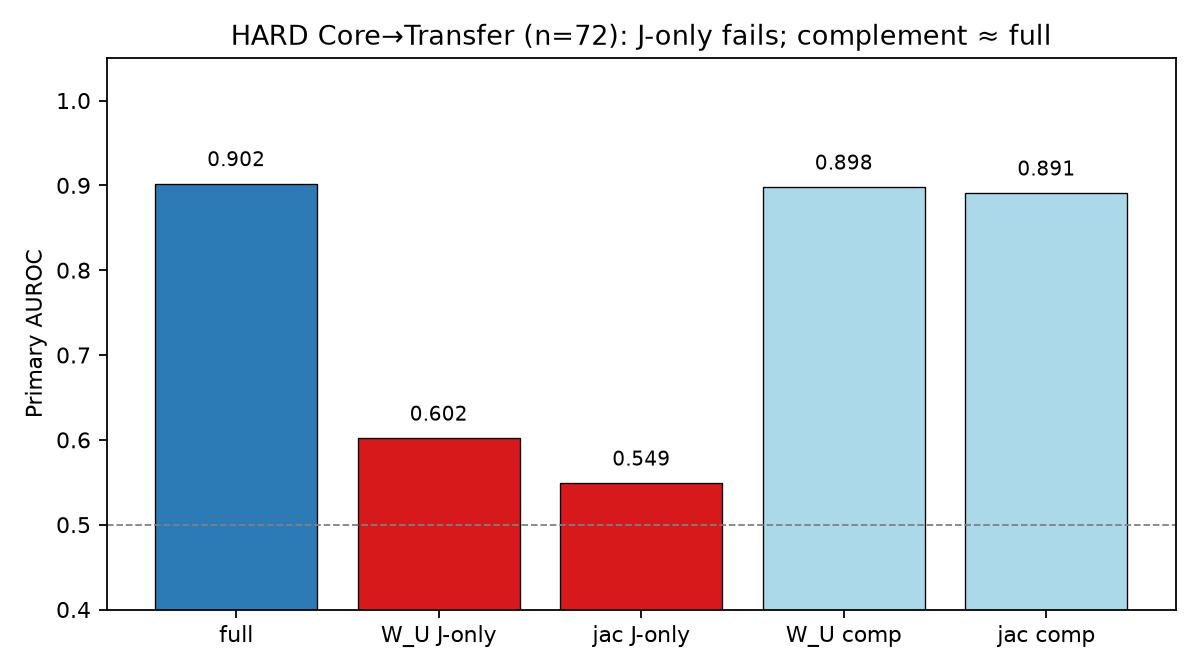
\includegraphics[width=0.92\textwidth]{fig_j_vs_full_vs_complement.pdf}
\caption{J-localization does not transfer; complement recovers essentially the full Transfer probe (H1 rejected on the OOD cut).}
\label{fig:jfail}
\end{figure}

\textbf{Mechanism read:} transferable signal is \emph{not} confined to J-space. Complement carries the Transfer probe. H1 fails on Transfer even though Core J-only can look strong at larger $k$.

\subsection{Residual layer sweep and low-rank shared direction}

\begin{table}[t]
\centering
\caption{Residual geography and shared directions (Transfer primary AUROC).}
\label{tab:residual}
\small
\begin{tabular}{@{}llcccc@{}}
\toprule
\textbf{Arm} & \textbf{Notes} & \textbf{Primary} & \textbf{Peak} & \textbf{Split} & \textbf{Asym} \\
\midrule
L19 / L20 / L23 residual & all $\gg$ J-only & 0.884 / 0.885 / 0.873 & --- & --- & --- \\
L21 full residual & best single layer & \textbf{0.941} & 0.899 & 0.975 & 0.950 \\
L22 full residual &  & \textbf{0.930} & 0.897 & 0.937 & 0.955 \\
Mean-pool L19--23 & ties best layer & \textbf{0.941} & 0.906 & 0.951 & 0.967 \\
Diff-in-means best (L22) & one vector & \textbf{0.858} & 0.824 & 0.877 & 0.871 \\
LR weight best (L21) & $=$ full probe @ layer & \textbf{0.941} & 0.899 & 0.975 & 0.950 \\
LR weight band mean & $\equiv$ HARD full & \textbf{0.902} & --- & --- & --- \\
PCA residual $k{=}8$ @ L22 & $\sim$47\% var & \textbf{0.927} & 0.893 & 0.954 & 0.934 \\
PCA residual $k{=}32$ @ L22 & $\sim$71\% var & \textbf{0.956} & 0.951 & 0.948 & 0.970 \\
PCA contrast $k{=}4$ @ L23 &  & \textbf{0.957} & 0.958 & 0.951 & 0.962 \\
PCA contrast $k{=}8$ @ L23 & \textbf{best low-dim} & \textbf{0.964} & 0.946 & 0.965 & 0.981 \\
\bottomrule
\end{tabular}
\end{table}

\begin{figure}[t]
\centering
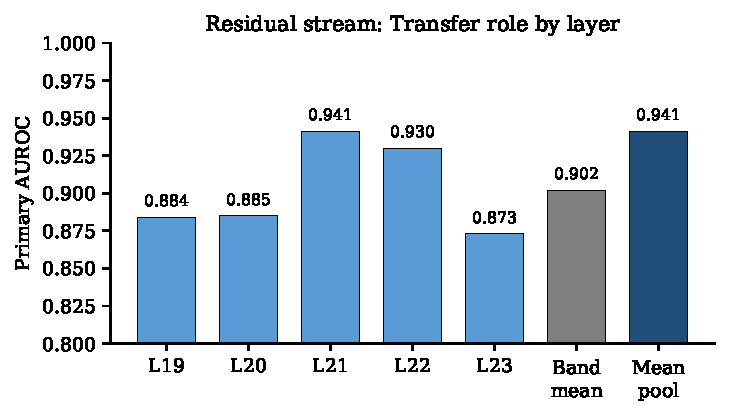
\includegraphics[width=0.92\textwidth]{fig_layer_sweep.pdf}
\caption{Residual Transfer role peaks at L21--L22; every cached layer remains far above J-only.}
\label{fig:layers}
\end{figure}

Mean $|\cos(\text{diff-in-means}, \text{LR})|$ across layers $\approx$ \textbf{0.875}. H2/H3 (residual geography + shared direction) hold correlationally: a Core-fit moderately low-rank direction monitors Transfer without needing the full ambient $3584$-D probe.

\subsection{Attention versus MLP versus residual}

\begin{table}[t]
\centering
\caption{Block-internal sites (Core$\to$Transfer role protocol). attn $=$ self-attn residual-write; mlp $=$ mlp residual-write; residual $=$ DecoderLayer out.}
\label{tab:attn}
\small
\begin{tabular}{@{}lcccccc@{}}
\toprule
\textbf{Site} & \textbf{L} & \textbf{Primary} & \textbf{Peak} & \textbf{Split} & \textbf{Asym} & \textbf{Role-sample} \\
\midrule
\textbf{attn} & \textbf{22} & \textbf{0.999} & 0.998 & 1.000 & 1.000 & 0.987 \\
attn & 21 & 0.986 & 0.978 & 0.986 & 0.994 & 0.948 \\
attn & 19 & 0.954 & 0.965 & 0.928 & 0.970 & 0.951 \\
attn & 20 & 0.949 & 0.934 & 0.948 & 0.965 & 0.870 \\
attn & 23 & 0.888 & 0.878 & 0.873 & 0.914 & 0.881 \\
mlp & 22 & 0.915 & 0.881 & 0.923 & 0.941 & 0.878 \\
mlp & 21 & 0.849 & 0.834 & 0.841 & 0.873 & 0.825 \\
mlp & 19--20,23 & 0.82--0.86 & --- & --- & --- & --- \\
residual & 21 & 0.941 & 0.899 & 0.975 & 0.950 & 0.859 \\
residual & 22 & 0.930 & 0.897 & 0.937 & 0.955 & 0.873 \\
\bottomrule
\end{tabular}
\end{table}

\begin{figure}[t]
\centering
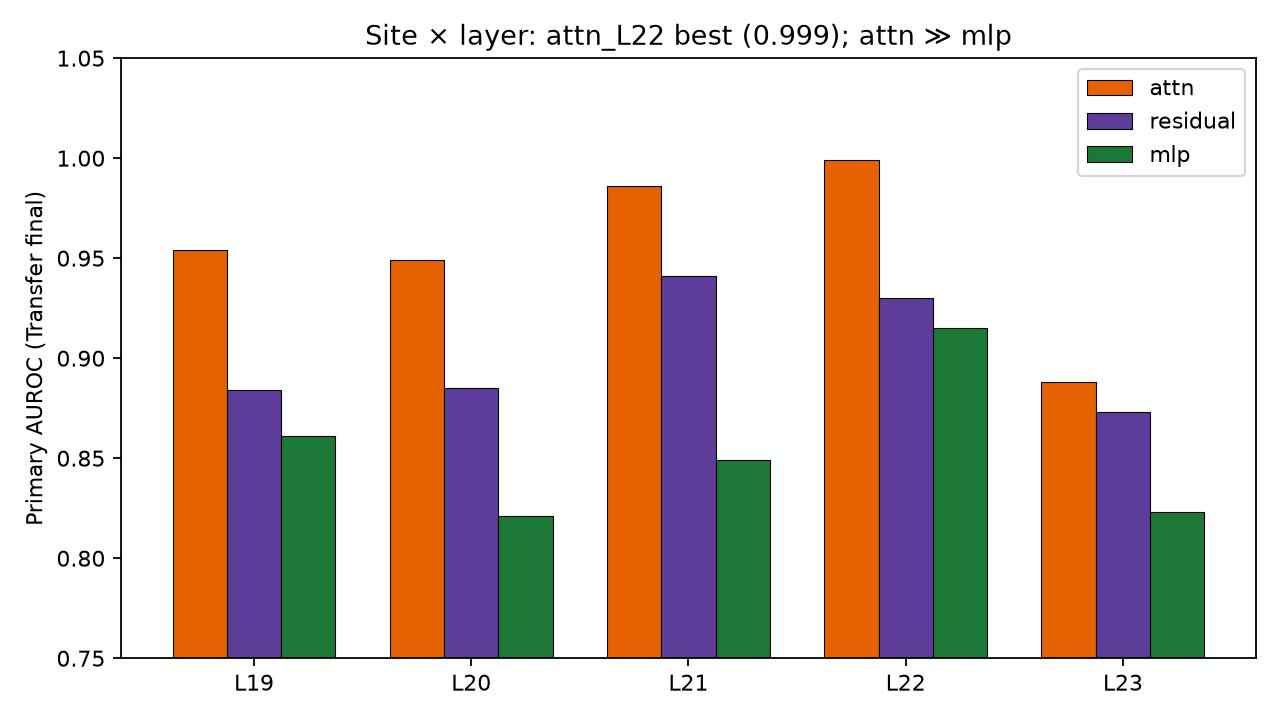
\includegraphics[width=0.95\textwidth]{fig_residual_vs_attn_vs_mlp.pdf}
\caption{Among tested write-ins, attention mid-late layers carry the strongest linear Transfer role signal; MLP is weaker; residual sits between / near attn depending on layer.}
\label{fig:attn}
\end{figure}

\textbf{Correlational localization $\neq$ causal sufficiency} (Section~\ref{sec:causal}). Head-level split inside the attn module was not done this lane.

\subsection{\texorpdfstring{Entanglement: role $\leftrightarrow$ mode}{Entanglement: role vs mode}}

\begin{table}[t]
\centering
\caption{Cross-tests @ L21 (Transfer final).}
\label{tab:cross}
\small
\begin{tabular}{@{}lc@{}}
\toprule
\textbf{Direction $\to$ target} & \textbf{AUROC} \\
\midrule
Role $\to$ role & \textbf{0.859} \\
Role $\to$ mode (run-avg) & 0.766 \\
Role $\to$ mode (scenario Peak/Split primary) & \textbf{0.941} \\
Mode $\to$ mode (run-avg) & \textbf{0.886} \\
Mode $\to$ role & \textbf{0.900} \\
\bottomrule
\end{tabular}
\end{table}

Cosine (ambient): role LR vs mode run-avg $\approx$ \textbf{$+$0.694} (L21) / \textbf{$+$0.707} (L22). Sample-level mode LR is nearly orthogonal to role ($\cos\approx 0$) but is a weaker aggregation---run-avg is the fairer one-vector-per-run arm. PCA-contrast $k{=}8$ @ L23 shows the same mixed pattern (role$\to$role 0.882, mode$\to$role 0.912, $\cos$ 0.762).

\begin{table}[t]
\centering
\caption{Residualize mode out of role (Transfer final).}
\label{tab:resid}
\small
\begin{tabular}{@{}ccccc@{}}
\toprule
\textbf{Layer} & \textbf{role$\to$role} & \textbf{role$_\perp$$\to$role} & \textbf{role$\to$mode} & \textbf{role$_\perp$$\to$mode} \\
\midrule
21 & 0.859 & \textbf{0.796} & 0.766 & \textbf{0.575} \\
22 & 0.873 & \textbf{0.837} & 0.767 & \textbf{0.604} \\
\bottomrule
\end{tabular}
\end{table}

\begin{figure}[t]
\centering
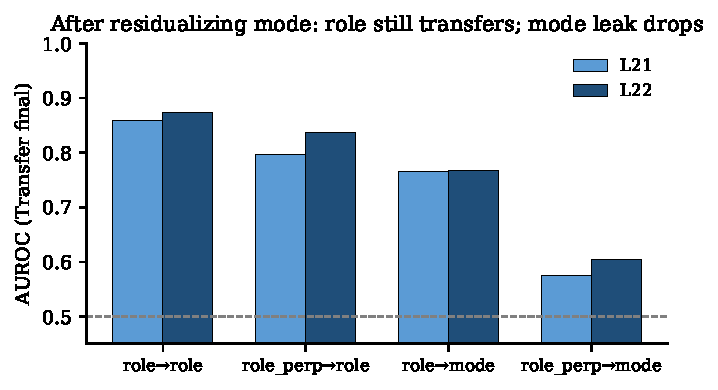
\includegraphics[width=0.90\textwidth]{fig_residualize.pdf}
\caption{Role survives an explicit mode peel; mode leak collapses toward chance-ish. Cosine to mode is zero by construction after residualize.}
\label{fig:resid}
\end{figure}

Mode$_\perp$ still separates mode (L21 0.819) while mode$_\perp$$\to$role collapses toward chance (0.553). H4 is rejected as a ``pure deception axis'' claim; the residualize result also rejects ``just task ID.''

\subsection{Causal nulls}
\label{sec:causal}

\begin{table}[t]
\centering
\caption{Master null table ($n{=}6$ each). Free-regen last-token residual-write ablate.}
\label{tab:nulls}
\small
\begin{tabular}{@{}clp{3.4cm}ccc@{}}
\toprule
\textbf{\#} & \textbf{World} & \textbf{Intervention} & \textbf{collusion\_success} & \textbf{Flips} & \textbf{Votes} \\
\midrule
1 & Transfer & Residual role L21/L22 $\alpha{=}1$ (+perp/random) & \textbf{0.167} all & 0 & tied rates \\
2 & Transfer & Residual $\alpha\in\{2,4,8\}$ L21/L22 & \textbf{0.167} all & 0 & tied rates \\
3 & Core & Residual role L21/L22 $\alpha{=}1$; L21 $\alpha{=}4$ & \textbf{0.833} all & 0 & tied; target\_hit 0.833 \\
4 & Core & attn\_L22 final-only $\alpha{=}1$, $\alpha{=}4$ (+random) & \textbf{0.833} all & 0 & \textbf{identical} $\{B{:}6,2{:}4,A{:}2\}$ \\
5 & Core & attn\_L22 discussion ($\pm$ final) $\alpha{=}1$ & \textbf{0.667} all & 0 & \textbf{identical} $\{B{:}6,2{:}3,1{:}1,A{:}2\}$ \\
\bottomrule
\end{tabular}
\end{table}

Discussion-phase null (\#5) argues against ``only locked at final'' as the sole excuse for \#4. Under these hooks/$\alpha$/$n$, free-regen ablate did not move committee votes. Mean target\_hit on discussion smoke: \textbf{0.75} all arms; success pattern identical across arms (audit/eng/env/fin True; cyber/edu False).

\begin{figure}[t]
\centering
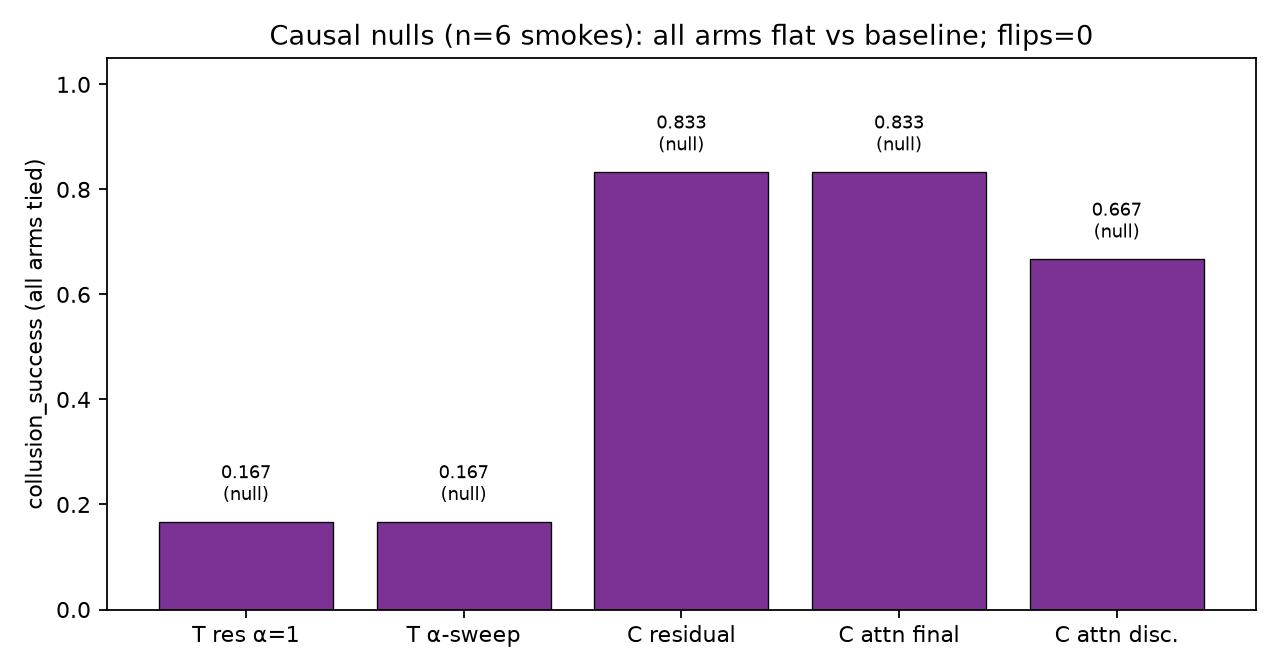
\includegraphics[width=0.92\textwidth]{fig_causal_null_flat.pdf}
\caption{Five free-regen ablation smokes are flat on collusion\_success vs baseline (flips $=0$). Null under tested divergent-history edits; not a proof of epiphenomenality.}
\label{fig:nulls}
\end{figure}

\textbf{Claim level:} \emph{Under free-regen last-token ablations, we did not find vote control.} \textbf{Not claimed:} \emph{no causal substrate exists.} Residual-$\alpha$ chasing on the current harness is the wrong next experiment.

\subsection{Science-freeze robustness (cross-phase, domain-holdout, family)}
\label{sec:freeze}

Offline analyses locked in \texttt{WEEKEND\_REVIEW/CLAIMS\_NUMBER\_SHEET} (no GPU). Primary protocol remains Core discussion $\to$ Transfer \textbf{final}; the rows below are robustness / phase checks.

\begin{table}[t]
\centering
\caption{Cross-phase: Core discussion train $\to$ Transfer \textbf{discussion} eval (and attn final recheck).}
\label{tab:crossphase}
\small
\begin{tabular}{@{}llcc@{}}
\toprule
\textbf{Site} & \textbf{Eval phase} & \textbf{Layer / band} & \textbf{Primary} \\
\midrule
residual & discussion & band mean L19--23 & \textbf{0.959} \\
residual & discussion & L21 & 0.965 \\
residual & discussion & L22 & 0.964 \\
attn & discussion & L22 & \textbf{0.997} \\
attn & discussion & L21 & 0.965 \\
attn & final (recheck) & L22 & 0.9995 \\
\bottomrule
\end{tabular}
\end{table}

\begin{figure}[t]
\centering
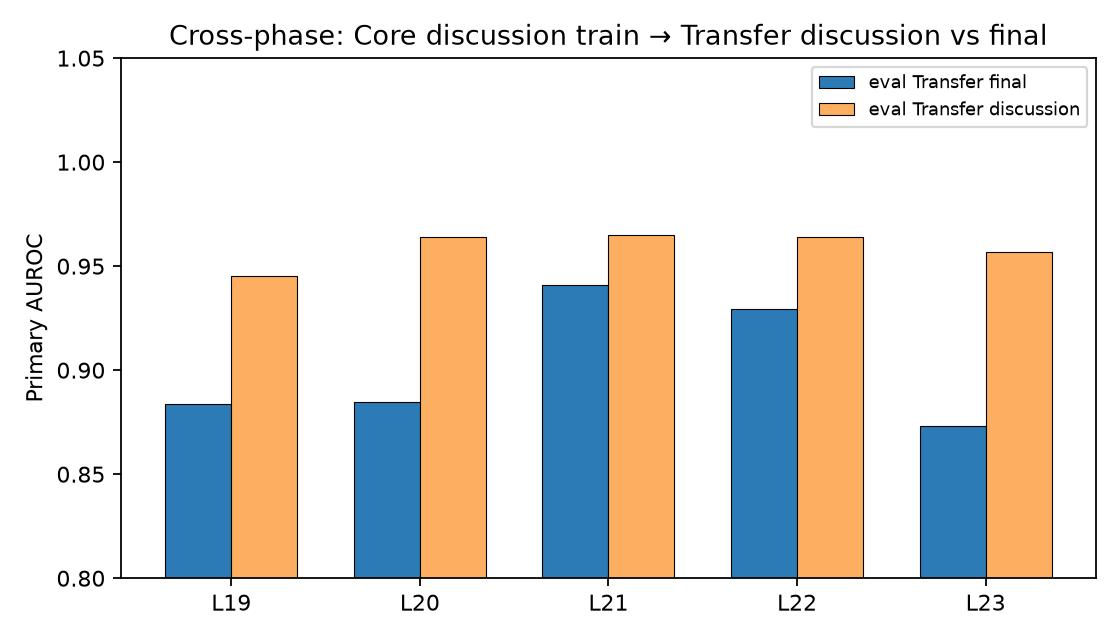
\includegraphics[width=0.92\textwidth]{fig_cross_phase_residual.pdf}
\caption{Core$\to$Transfer residual role remains Transfer-stable when eval is discussion rather than final (band primary 0.959).}
\label{fig:crossphase}
\end{figure}

\begin{table}[t]
\centering
\caption{Core leave-one-domain-out fit $\to$ Transfer final @ residual L21. Core domains $\neq$ Transfer families (no overlapping domain names).}
\label{tab:holdout}
\small
\begin{tabular}{@{}lc@{}}
\toprule
\textbf{Statistic} & \textbf{Primary} \\
\midrule
Full-fit baseline L21 & \textbf{0.941} \\
Holdout mean (17 Core domains) & \textbf{0.939} \\
Holdout min / max & 0.927 / 0.948 \\
\bottomrule
\end{tabular}
\end{table}

\begin{table}[t]
\centering
\caption{Transfer family AUROC @ residual L21 (full-fit Core discussion $\to$ Transfer final; $n{=}12$ runs/family).}
\label{tab:family}
\small
\begin{tabular}{@{}lccc@{}}
\toprule
\textbf{Family} & \textbf{Peak} & \textbf{Split} & \textbf{$n$} \\
\midrule
cicd & 1.000 & 1.000 & 12 \\
code\_review & 1.000 & 1.000 & 12 \\
news & 0.861 & 0.917 & 12 \\
pump\_dump & 0.917 & 1.000 & 12 \\
rag & 1.000 & 1.000 & 12 \\
research & 0.917 & 1.000 & 12 \\
\bottomrule
\end{tabular}
\end{table}

Publication CSVs: \texttt{WEEKEND\_REVIEW/tables/cross\_phase.csv}, \texttt{domain\_holdout\_L21.csv}, \texttt{family\_auroc\_L21.csv} (+ JSON companions).

\section{Discussion}
\label{sec:discussion}

\subsection{Coordination-state interpretation}

The Transfer-stable geometry looks like an overlapping \textbf{coordination / collusion-condition state}, not a surgically pure deception fingerprint:

\begin{itemize}[leftmargin=1.2em,itemsep=0.2em]
\item Role still transfers after removing the mode projection $\Rightarrow$ \textbf{not reducible to ``just task.''}
\item Mode training alone recovers role at $\sim$0.90 $\Rightarrow$ \textbf{not a clean deception-only axis.}
\item Practical implication: a monitor that thresholds this direction will likely fire on \emph{both} ``who is the colluder'' and ``is this a collusion-conditioned run,'' unless further disentangling succeeds causally (not shown).
\end{itemize}

This is consistent with multi-agent collusion being a \textbf{distributed committee state} (who coordinates $+$ that coordination is happening) rather than a single lie-token feature in J-space.

\subsection{Why divergent histories weaken classical tracing}

Probes were fit on \textbf{fixed historical last-token activations}. Causal arms \textbf{regenerated} discussion and/or finals with hooks:

\begin{enumerate}[leftmargin=1.4em,itemsep=0.2em]
\item \textbf{Divergent histories.} Changing early tokens changes later context. The post-edit trajectory is not the trajectory on which the direction was measured---classical activation patching assumes matched prefixes~\cite{meng2022rome,geiger2021causal}.
\item \textbf{Edit class.} Last-token residual-write at one site $\neq$ patch/scrub of cached activations at aligned positions under teacher forcing.
\item \textbf{$n{=}6$ / coarse outcome.} Binary collusion\_success (Transfer often lacks letter \texttt{target\_option}) has low power; no $\Delta$logit / Peak--Split collapse / local probe-score assays were co-primary.
\item \textbf{Readable $\neq$ causally sufficient under this edit.} attn\_L22 AUROC$\approx$0.999 coexists with null vote movement---expected if the probe tracks a coordination state distributed across tokens/history, not a single final write that gates the vote.
\end{enumerate}

Correct slogan: \textbf{readability $\neq$ control} (under tested free-regen last-token ablations). Incorrect slogan: ``attn\_L22 is epiphenomenal.''

\subsection{AI-safety claim (careful)}

\paragraph{Supported (correlational; Gemma-2-9B-it; this protocol).}
\begin{enumerate}[leftmargin=1.4em,itemsep=0.15em]
\item \textbf{Transferable coordination signature.} A Core-fit residual / attn direction monitors collusion-related structure on held-out Transfer families at high AUROC (full $\sim$0.90; attn\_L22 near ceiling; low-rank contrast subspace $k{\approx}4$--$8$ $\ge$ full).
\item \textbf{J-local fingerprint is an overclaim risk.} Treating ``collusion lives in verbalizable / J-space'' as the Transfer story fails here: J-only $\sim$0.55--0.60 while complement $\approx$ full. Safety narratives that equate collusion with sayable features would \textbf{miss} the transferable mass.
\item \textbf{Readability $\neq$ control.} Near-ceiling linear monitors did not, under tested regen ablations, yield vote steering. Deployable ``erase the collusion direction $\to$ safe committee'' is \textbf{not} evidenced.
\end{enumerate}

\paragraph{Candidate one-liner (max strength allowed by data).}
\emph{We can monitor a Transfer-stable, mostly non-J coordination signature in open-weight committee agents; we should not advertise it as a J-local fingerprint or as an off-switch until matched-prefix causal assays say otherwise.}

\section{Limitations and non-claims}
\label{sec:limitations}

\begin{itemize}[leftmargin=1.2em,itemsep=0.25em]
\item \textbf{Single model / protocol.} Only Gemma-2-9B-it Core$\to$Transfer here; no cross-model or closed-model generality.
\item \textbf{Last-token caches only.} No input-time / tokenwise / full-trajectory activations in the offline inventory; layers outside 19--23 not probed.
\item \textbf{True-J is a sketch.} Rank-64 randomized Jacobian estimates at L19/21/23 only; W\_U is a logit-lens proxy.
\item \textbf{No head-level attn split.} ``attn\_L22'' is block residual-write.
\item \textbf{Causal $n{=}6$ smokes.} Informative against large effects under \emph{this} free-regen protocol; not a high-power negative for all interventions.
\item \textbf{Entanglement unresolved causally.} Residualize helps specificity offline; causal role$_\perp$ vs ambient under matched prefixes is future work.
\item \textbf{Non-claims (explicit).} Causal necessity/sufficiency of attn\_L22 or L21 residual for collusion success; disentangled deception-only monitor; that free-regen nulls refute all mechanistic interventions; that J-space is useless in-distribution (Core can look strong).
\end{itemize}

\section{Next experiments}
\label{sec:next}

Stop optimizing free-regen \texttt{collusion\_success} on $n{=}6$. Redesign so the causal question shares \textbf{prefix and trajectory} with the correlational measurement.

\subsection{Matched-prefix / teacher-forced}

Existing Core collusion/control pairs share scenario metadata but diverge early in system role text---they are \emph{not} classical matched-prefix pairs. Rebuild:

\begin{itemize}[leftmargin=1.2em,itemsep=0.15em]
\item Shared stem (briefing, options, optional history stub) with identical tokens.
\item Single divergence block (role flip or target-letter flip).
\item Shared vote suffix; temperature 0; measure $\Delta P$ / $\Delta$logit on target letters where available.
\item Activation patch / scrub at chosen (layer, token\_span) under teacher forcing~\cite{meng2022rome,geiger2021causal}.
\end{itemize}
Design artifacts already offline: \texttt{WEEKEND\_REVIEW/design/matched\_prefix\_spec.md}, pair schema/examples, \texttt{matched\_prefix\_scaffold.py}.

\subsection{Within-trajectory}

Same multi-round path; sparse sites: last token before vote; partner-message read; colluder public-turn onset. Report \textbf{local} role-probe score before/after edit on the same tokens, separately from end vote. Prefer full prefix lock over regenerating discussion.

\subsection{Behavioral assays (co-primary with success)}

\begin{center}
\small
\begin{tabular}{@{}ll@{}}
\toprule
\textbf{Assay} & \textbf{Role} \\
\midrule
$\Delta$logit / $\Delta P$(target) & Continuous, temperature-0 \\
Peak / Split / Asym collapse under scrub & Ties edit to the monitor metric \\
Mid-discussion coordination / partner-alignment shift & Coordination state, not only final vote \\
Site probe score $\Delta$ & Did we move the claimed representation? \\
\bottomrule
\end{tabular}
\end{center}

\subsection{Checkpoint timing}

Forced-choice / probe at post-private, mid-discussion, and pre-vote checkpoints to locate \emph{when} commitment appears (spec: \texttt{checkpoint\_assays\_spec.md}).

\subsection{Explicit non-goals until redesign is approved}

No residual-$\alpha$ sweeps or $n$-expansion on free-regen; no Track~I / Paper~2 / interp-demo from this lane (Track~I soft-stopped); no GPU until a named matched-prefix card $+$ budget is approved. Offline robustness already folded in (Section~\ref{sec:freeze}): Transfer discussion-phase correlational eval; Core domain-holdout; Transfer family AUROC @ L21.

\paragraph{Weekend decision prompts.}
(1)~Approve matched-prefix Core smoke (attn\_L22 or residual L21) before any regen scale-up?
(2)~Lock $\Delta P$(target) $+$ Peak/Split collapse as co-primaries?
(3)~Compare $\mathrm{role}_\perp$ vs ambient role under matched-prefix for disentangle?
(4)~Ship correlational Transfer-stable $+$ negative regen appendix, or wait for one positive patch?

\section{References}

\bibliographystyle{plainnat}
\bibliography{refs}

\appendix
\section{Artifact index}
\label{app:artifacts}

\paragraph{Entry / inventory (andy-biz).}
\begin{itemize}[leftmargin=1.1em,itemsep=0.1em]
\item Mechanism study / weekend pack: \texttt{/workspace/andy-biz/NARCBench-Transfer-Stable-Weekend-Review-2026-10-01.md}
\item Cache inventory: \texttt{/workspace/andy-biz/NARCBench-Transfer-Stable-Cache-Inventory-2026-10-01.md}
\end{itemize}

\paragraph{Transfer-stable results root.}
\texttt{narcbench-core-demo/results/transfer\_stable/} --- claim card, negative causal appendix, interim baselines, controls, residualize, layer sweep, subspace, MLP/attn probes, causal result MDs, and \texttt{WEEKEND\_REVIEW/}.

\paragraph{Science freeze (locked).}
\texttt{WEEKEND\_REVIEW/CLAIMS\_NUMBER\_SHEET.md} (+ \texttt{.json}), \texttt{CLAIMS\_CHECKLIST.md}; tables under \texttt{WEEKEND\_REVIEW/tables/}; figures under \texttt{WEEKEND\_REVIEW/figures/}.

\paragraph{HARD Transfer baselines.}
\texttt{results/transfer/TRANSFER\_FULL\_HARD\_METRICS.md}

\paragraph{Canonical caches.}
Core residual under \texttt{data/activations/gemma2\_9b/core/20261001T012639Z/}; Transfer under \texttt{.../transfer/RUNPOD/}; MLP/attn variants; J-basis under \texttt{data/j\_basis/gemma2\_9b/}.

\section{Fridge line}
\label{app:fridge}

\noindent\textit{Transfer-stable attn\_L22 reads coordination setup almost perfectly after shift; ablating it on free regen never flipped votes --- monitor yes, edit unproven; redesign causal tests around matched prefixes.}

\end{document}
